\chapter{Исследовательский раздел}

\section{Примеры построения деревьев составляющих}

Примеры деревьев зависимостей построенных для предложений романа Л.~Н. Толстого <<Война и мир>> показаны на рисунках~\ref{fig:tree_great} и~\ref{fig:tree_bad}.

\begin{figure}[H]
	\centering
	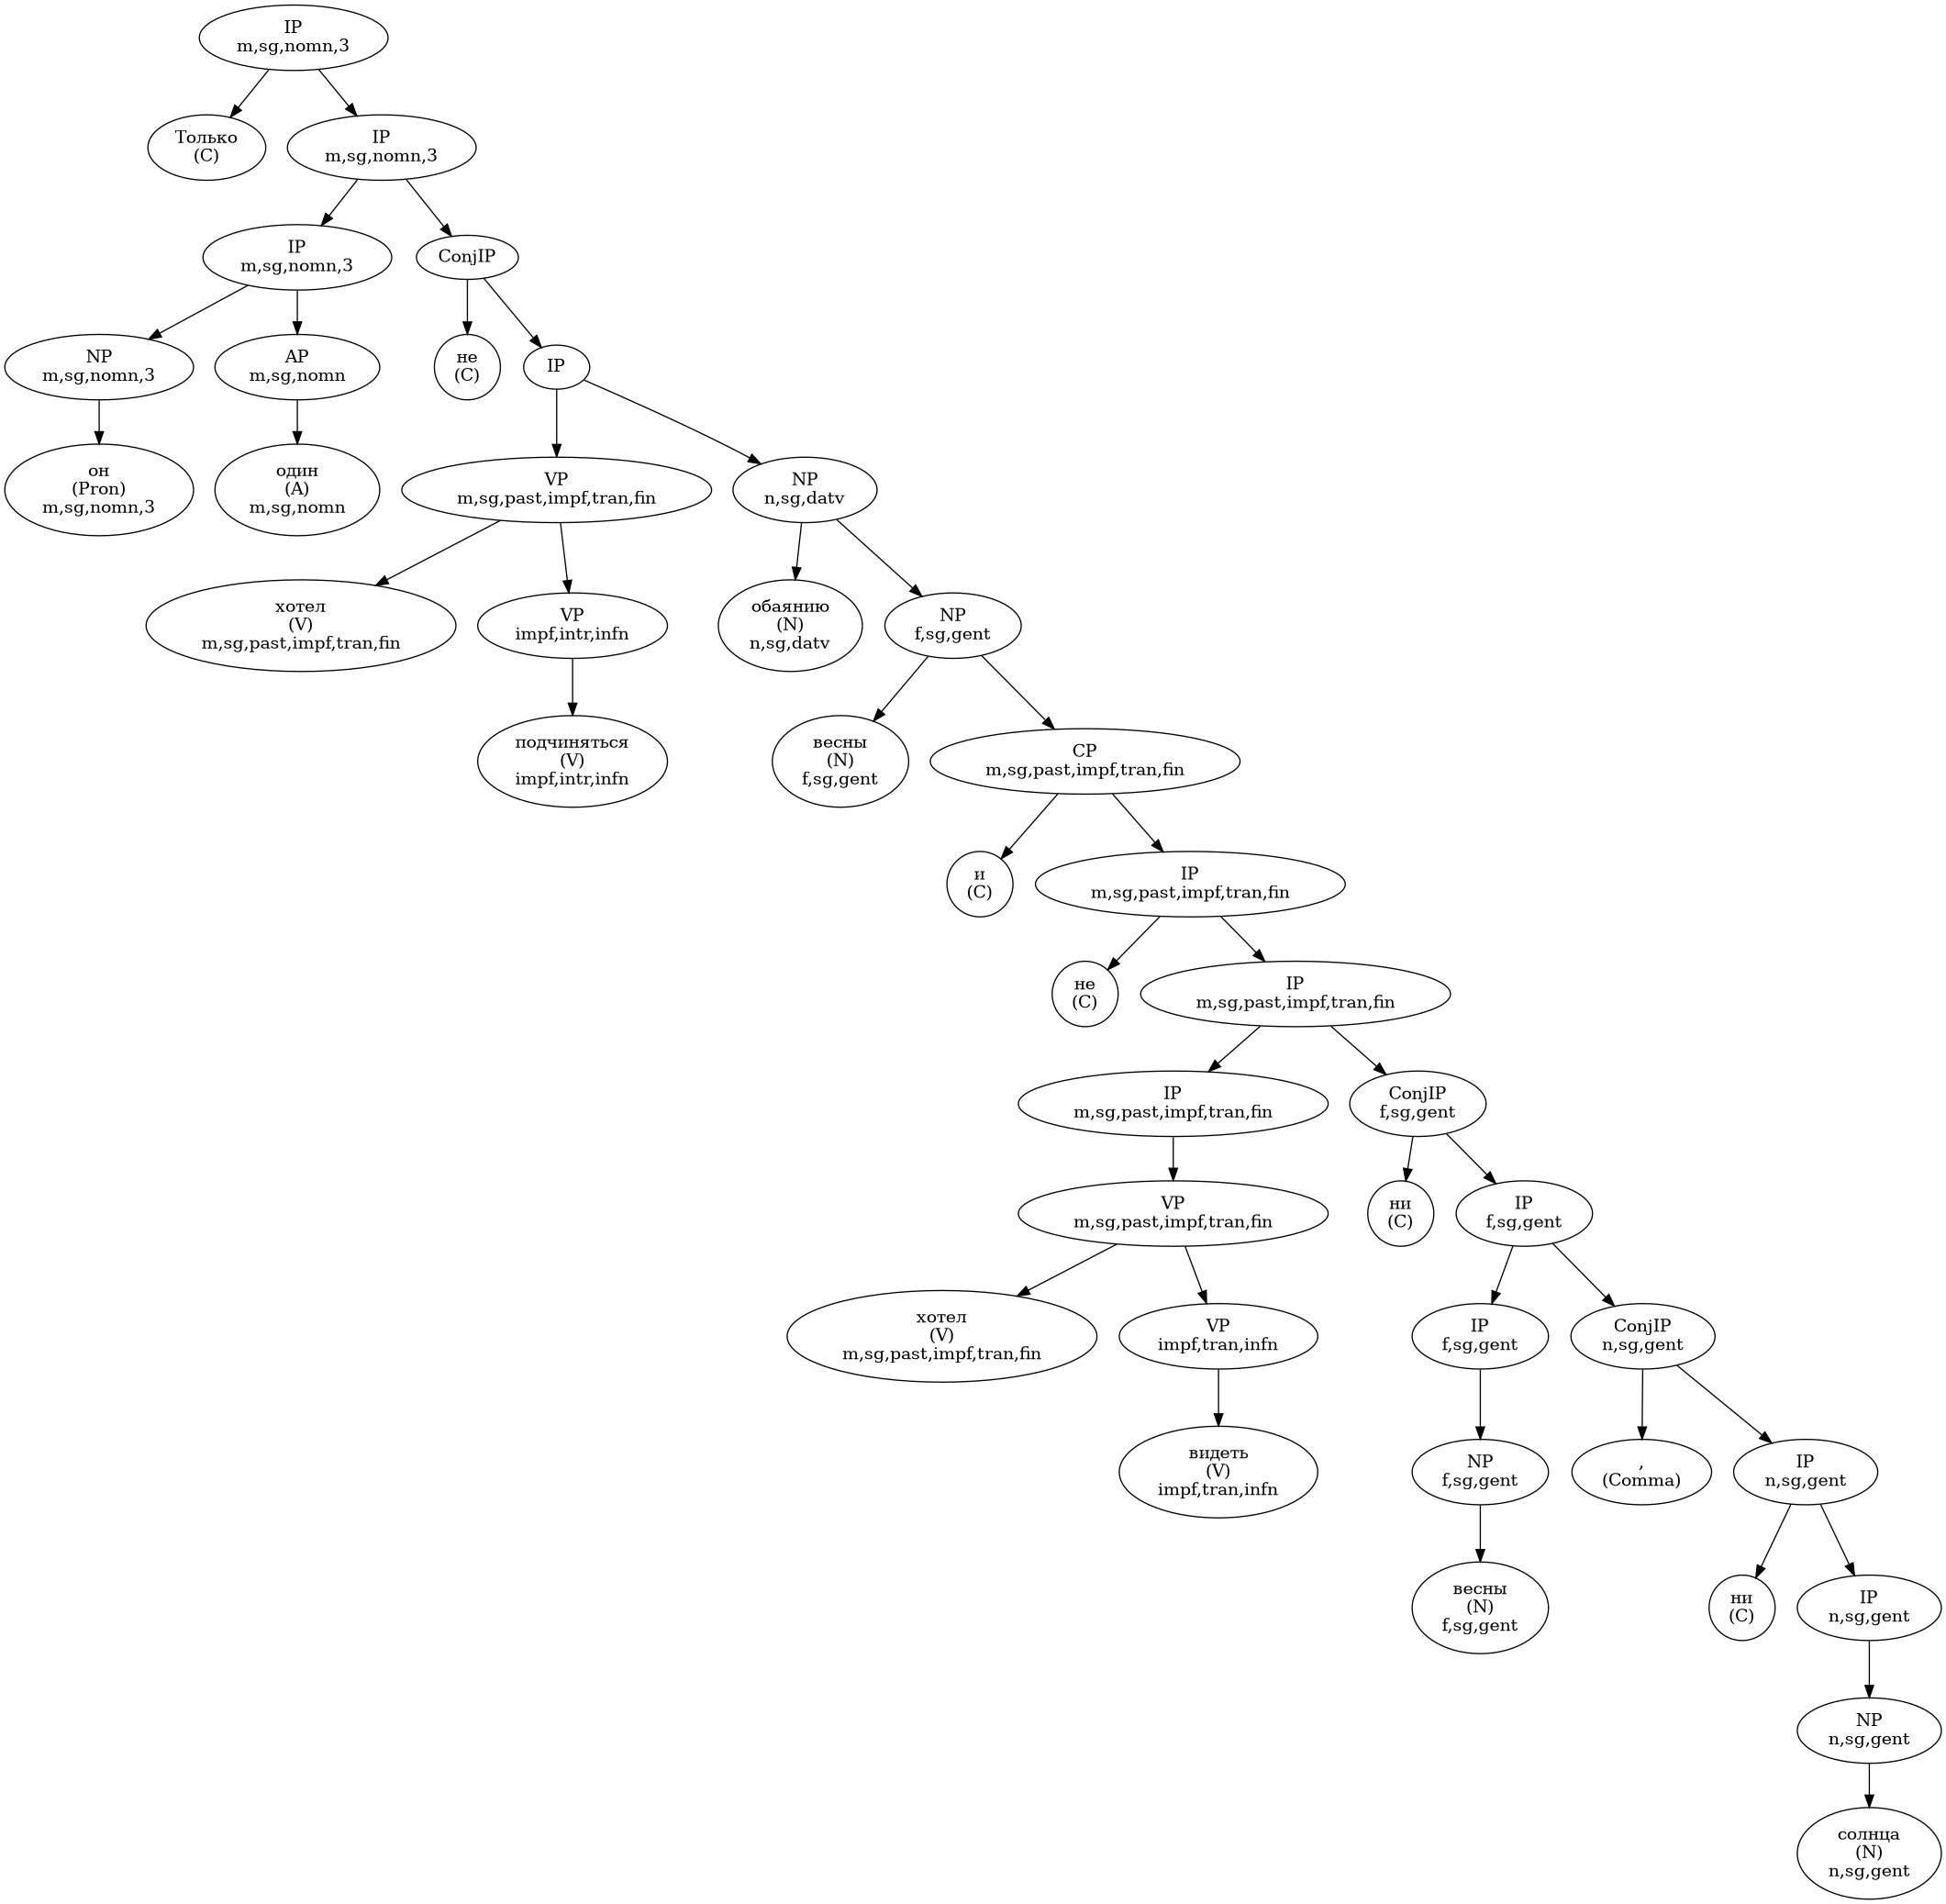
\includegraphics[width=\linewidth]{images/tree_great.png}
	\caption{Пример дерева составляющих для предложения <<Только он один не хотел подчиняться обаянию весны и не хотел видеть ни весны, ни солнца.>>}
	\label{fig:tree_great}
\end{figure}
\begin{figure}[H]
	\centering
	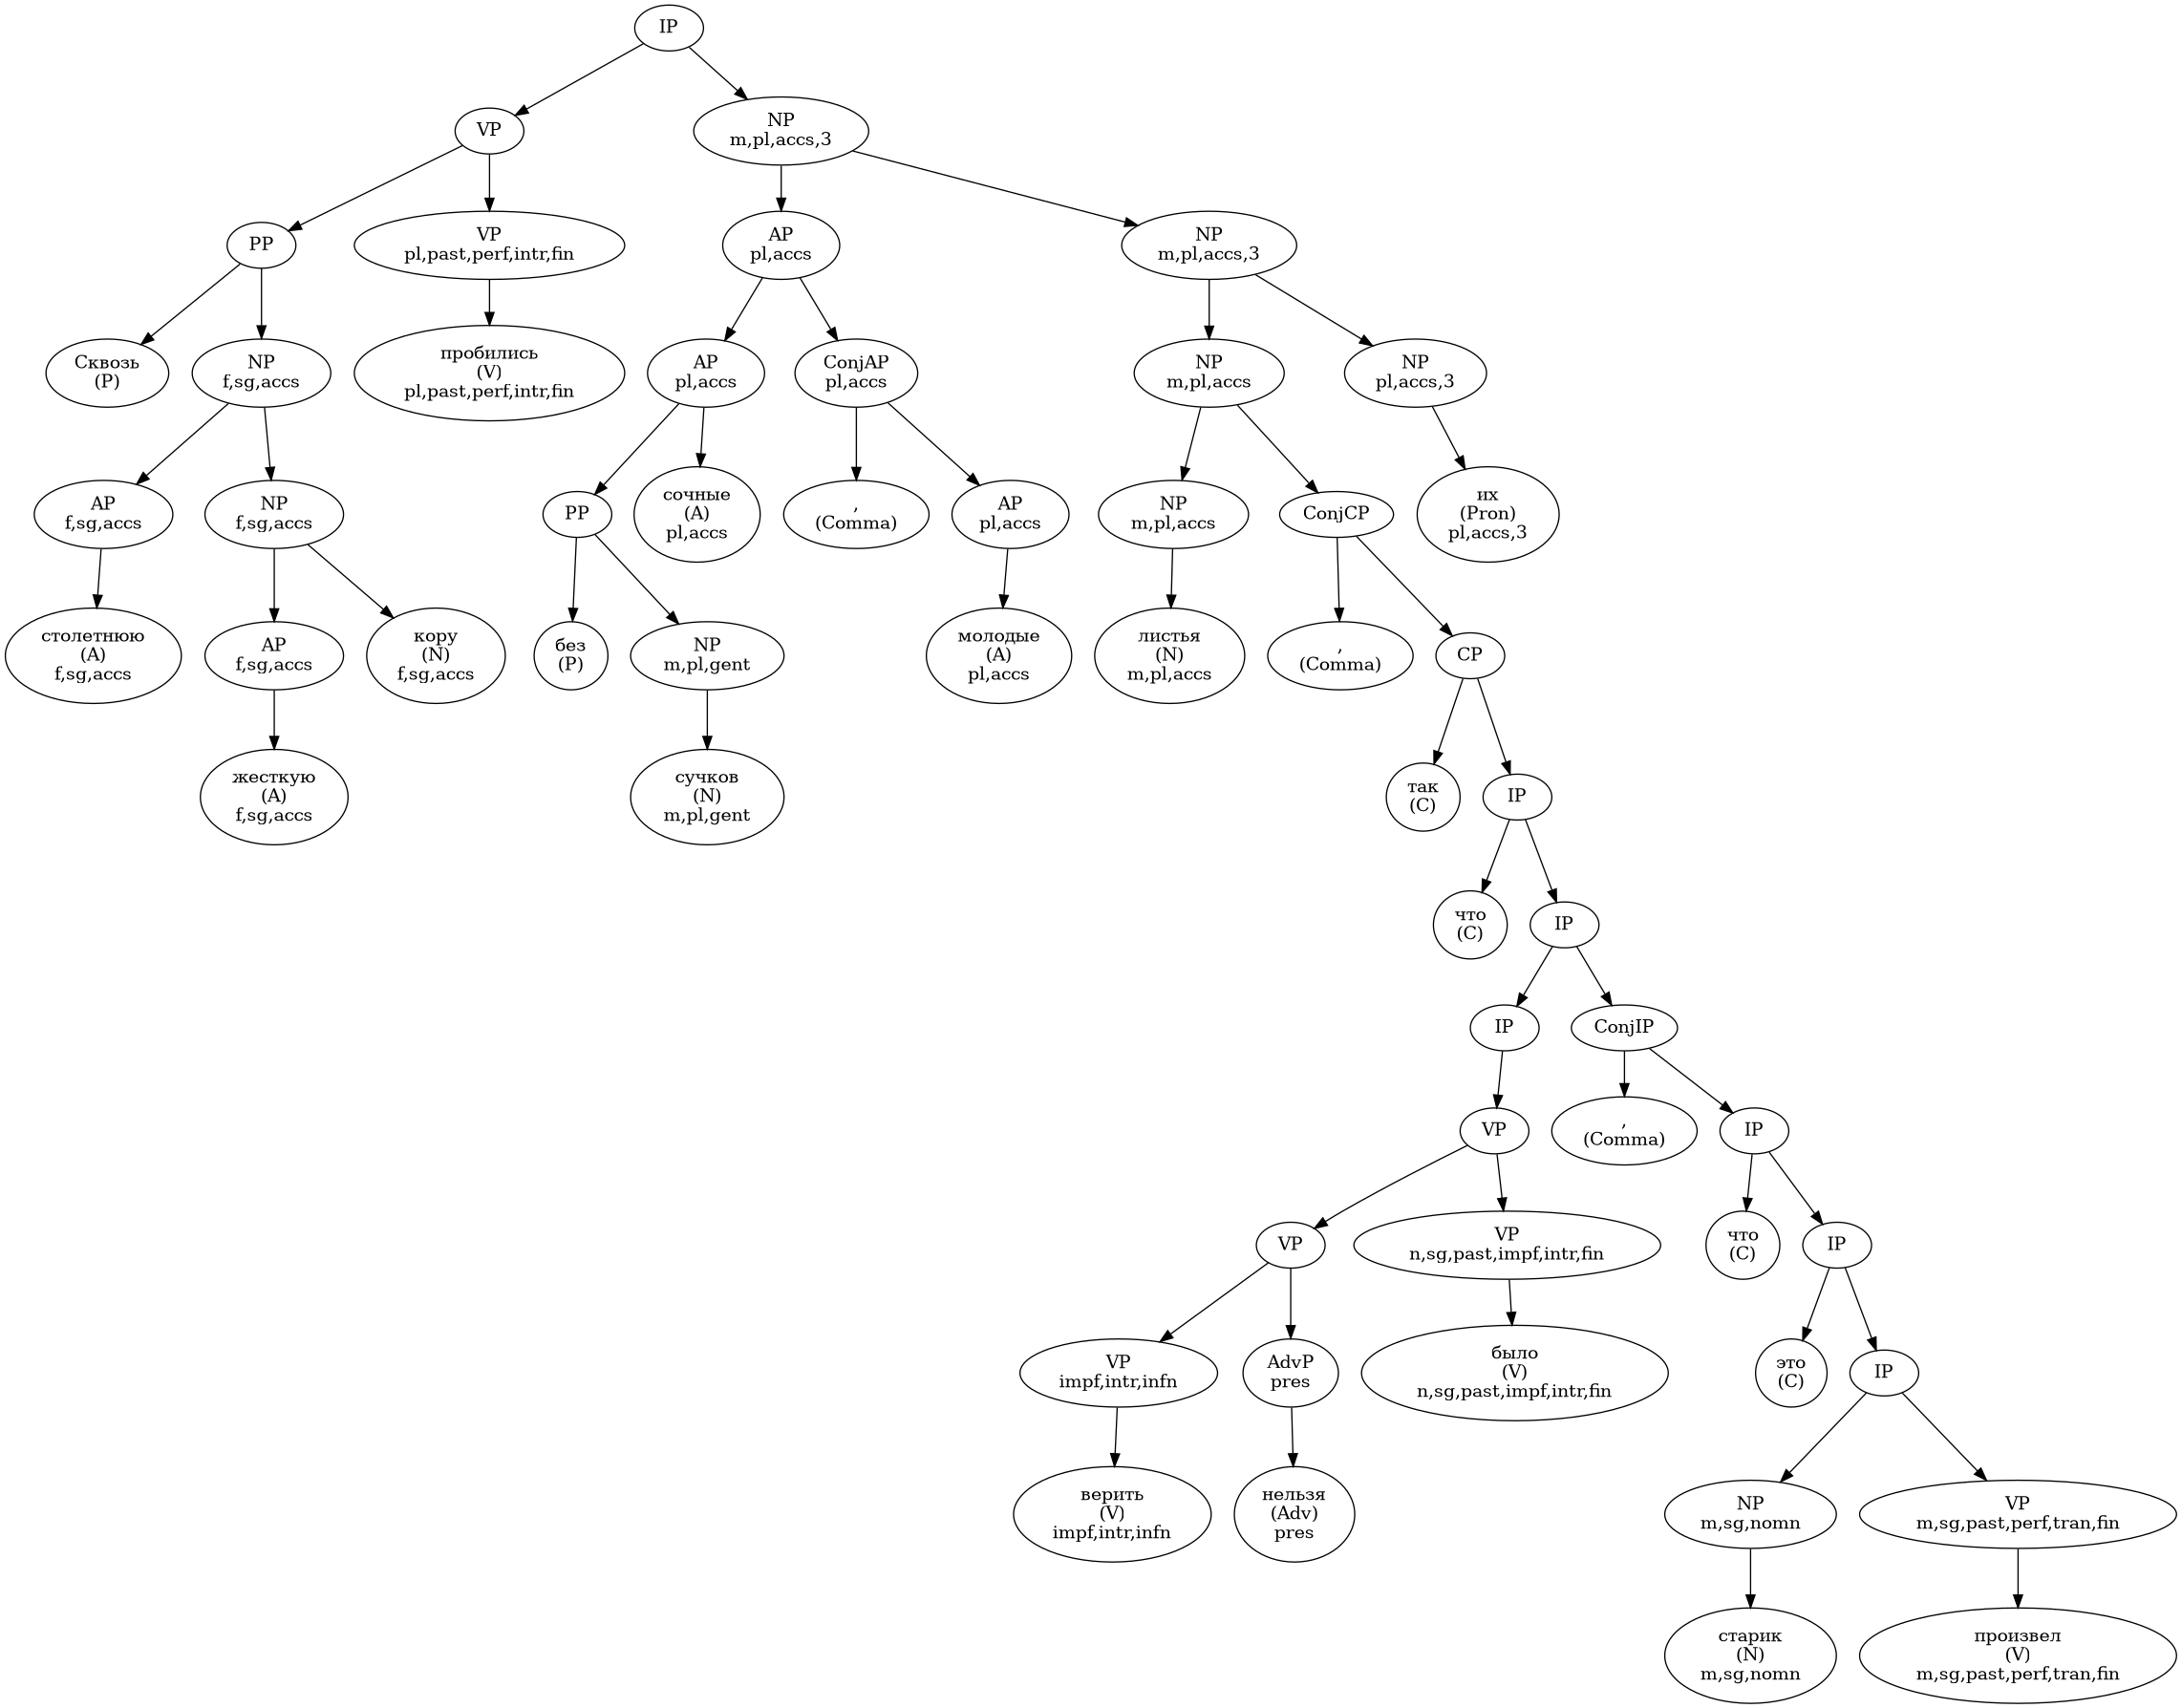
\includegraphics[angle=90, width=\linewidth]{images/tree_bad.png}
	\caption{Пример дерева составляющих для предложения <<Сквозь столетнюю жесткую кору пробились без сучков сочные, молодые листья, так что верить нельзя было, что это старик произвел их.>>}
	\label{fig:tree_bad}
\end{figure}
\section{Постановка исследования}

Исследования проводились на машине со следующими характеристиками:
\begin{itemize}[label=---]
	\item процессор Intel(R) Core(TM) i5-10210U~\cite{intel_i5_10210u_specs}, тактовая частота 1.60 ГГц, 8 логических ядер;
	\item оперативная память: 16~ГБ;
	\item операционная система: Ubuntu 24.04 LTS~\cite{ubuntu_24_04_docs}.
\end{itemize}

Задачами данного исследования являются:
\begin{itemize}
	\item получение зависимости времени выполнения ключевых этапов разработанного метода от числа словоформ во входном предложении;
	\item получение оценки точности и полноты разработанного метода.
\end{itemize}

Для получения зависимости времени выполнения ключевых этапов разработанного метода от числа словоформ в предложении, были проведены серии из 500 замеров для каждого числа $n$ словоформ в предложении. В данном случае в число словоформ включаются знаки препинания, поскольку в разработанном методе они анализируются аналогично служебным членам предложения. Для проведения замеров были сформулированы 20 предложений, состоящие из $n=\overline{1,20}$ словоформ. Верхний предел числа словоформ был выбран на основе среднего числа словоформ в современных художественных текстах равного 8 и 20 в юридических текстах~\cite{knutov2020complexity}.

Для оценки точности и полноты получаемых разработанным методом деревьев составляющих были использованы данные корпуса RuConst~\cite{Grashchenkov2024RuConst,grapaul_Ru_Const}. Основной единицей сравнения приведенных в корпусе деревьев составляющих и получаемых разработанным методом была выбрана тройка:
\begin{equation}
	\label{eq:compare}
	\langle l,\ i,\ j\rangle,
\end{equation}
где 
\begin{itemize}
	\item $l$~---~метка составляющей;
	\item $i$~---~индекс первой словоформы составляющей в исходном предложении;
	\item $j$~---~индекс последней словоформы составляющей в исходном предложении.
\end{itemize}

Поскольку в используемом в качестве эталонного корпусе множество меток состоит из $NP,\ VP,\ PP$, метки, получаемые разработанных методом, отличные от перечисленных не учитываются в сравнении.

Используемый в качестве эталонного корпус содержит единственное дерево составляющих для каждого предложения. Для проведения сравнения, среди всех получаемых разработанным методом деревьев составляющих выбирается единственное. Число совпавших с эталонным деревом троек~\ref{eq:compare} максимально для выбранного дерева.

Таким образом, если $G$~---~множество троек вида~\ref{eq:compare} дерева составляющих эталонного корпуса, $P$~---~множество троек вида~\ref{eq:compare} выбранного для сравнения дерева, построенного разработанным методом, то полнота, точность, $F1$-мера определяются следующим образом:

\begin{align}
	\label{eq:precision}
	\text{Precision} &= 
	\begin{cases}
		\dfrac{TP}{FP+TP}, & TP+FP \neq 0\\[6pt]
		0, & TP+FP = 0
	\end{cases}; \\
	\label{eq:recall}
	\text{Recall} &= 
	\begin{cases}
		\dfrac{TP}{FN+TP}, & TP+FN \neq 0\\[6pt]
		0, & TP+FN = 0
	\end{cases}; \\
	\label{eq:f1}
	F1 &= \frac{2 \cdot \text{Precision} \cdot \text{Recall}}{\text{Precision} + \text{Recall}},
\end{align}

где\begin{itemize}
	\item $TP = |G \cap P|$~---~тройки~\ref{eq:compare}, совпавшие в эталонном дереве составляющих и в полученном разработанным методом;
	\item $FP = |P \setminus G|$~---~тройки~\ref{eq:compare}, присутствующие в полученном разработанным методом дереве составляющих, но отсутствующие в эталонном;
	\item $FN = |G \setminus P|$~---~тройки~\ref{eq:compare}, присутствующие в эталонном дереве составляющих, но отсутствующие в полученном разработанным методом.
\end{itemize}

Результирующие значения точности, полноты и F1-меры вычисляются как среднее арифметическое по результатам выражений~\ref{eq:precision},~\ref{eq:recall} и~\ref{eq:f1} для 500 предложений корпуса~\cite{grapaul_Ru_Const}, количество словоформ в которых не превосходит 15.

\section{Результаты исследования}

Зависимость медианного время построения таблицы составляющих от числа словоформ в исходном предложении представлена на рисунке~\ref{fig:cyk_time}

\begin{figure}[H]
	\centering
	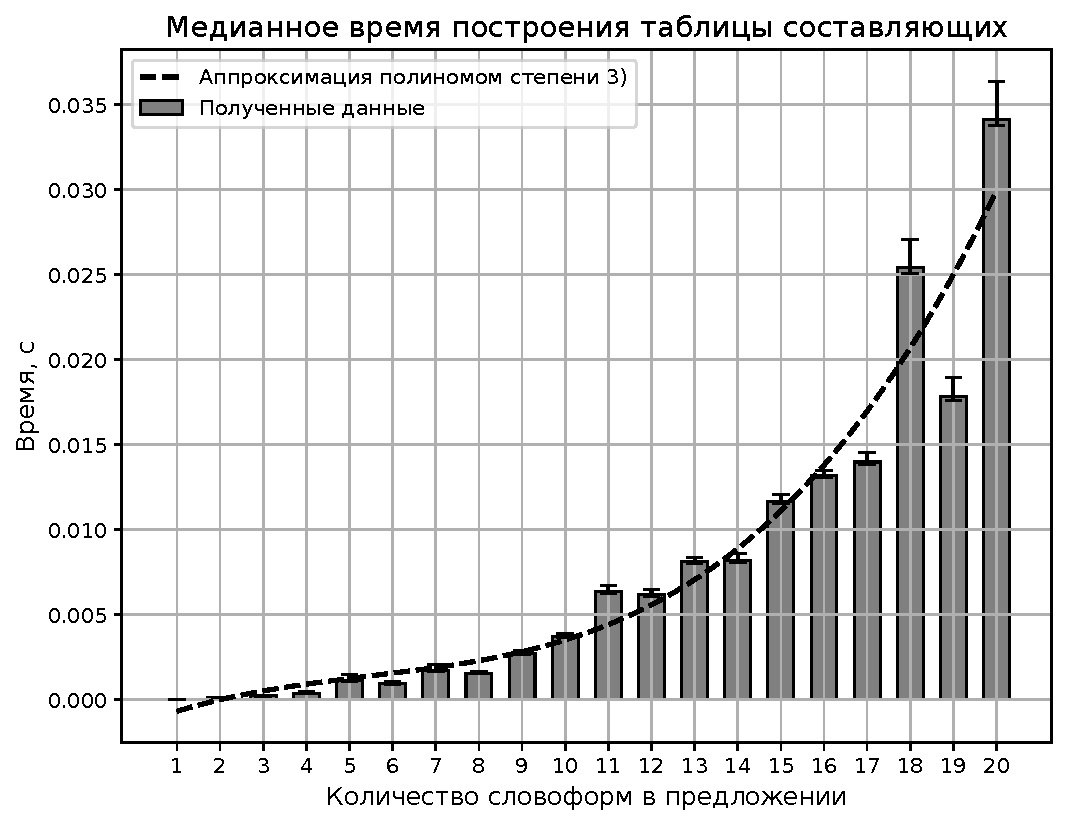
\includegraphics[width=\linewidth]{images/benchmark_cyk_hist.pdf}
	\caption{Зависимость медианного времени выполнения алгоритма построения таблицы составляющих от числа словоформ во входном предложении}
	\label{fig:cyk_time}
\end{figure}

Полученные данные были аппроксимированы полиномом третьей степени:
\begin{equation}
	\label{eq:cyk_approx}
	T_{table}(n) \approx 7.85 \cdot 10^{-6} n^3 -1.29\cdot 10^{-4}n^2+1.01\cdot 10^{-3}n-1.56\cdot 10^{-3}\text{,}
\end{equation}
где $n$~---~число словоформ в предложении.

Коэффициенты полинома были получены по методу наименьших квадратов, степень полинома была определена с помощью информационного критерия Акаике~\cite{burnham2002model}. В качестве альтернативных моделей рассматривались полиномы со степенями от 1 до 4. 

Зависимость медианного времени восстановления всех деревьев составляющих для исходного предложения с данным числом словоформ представлена на рисункe~\ref{fig:tree_time} в логарифмической шкале
\begin{figure}[H]
	\centering
	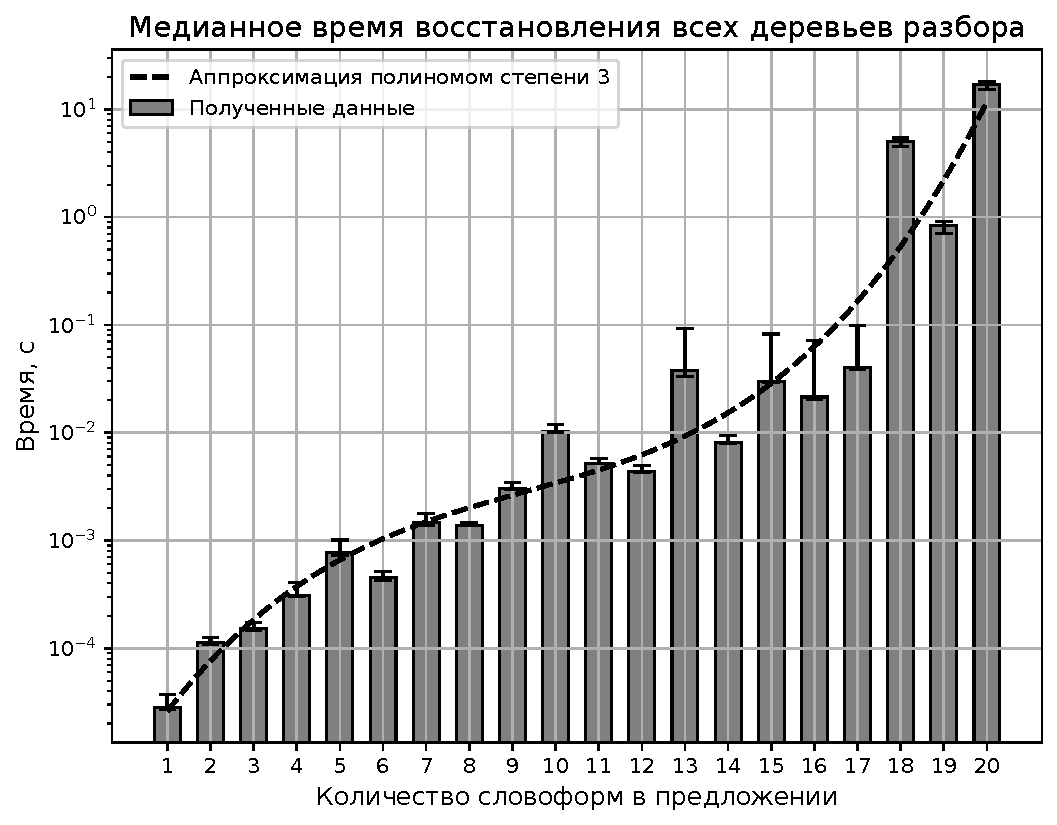
\includegraphics[width=\linewidth]{images/benchmark_trees_total_log_hist.pdf}
	\caption{Зависимость медианного времени выполнения алгоритма восстановления всех деревьев составляющих от числа словоформ во входном предложении}
	\label{fig:tree_time}
\end{figure}

Полученные данные были аналогично аппроксимированы полиномом третьей степени:
\begin{equation}
	\label{eq:tree_approx}
	T_{tree}(n) \approx 4.52 \cdot 10^{-3} n^3 -1.26\cdot 10^{-1}n^2+1.42n-11.86\text{.}
\end{equation}

В таблице~\ref{tab:trees_cnt} приведена также зависимость числа полученных деревьев составляющих от количества словоформ во входном предложении.

\begin{table}[H]
	\centering
	\caption{Зависимость числа восстановленных деревьев от числа словоформ в исходном предложении}
	\begin{tabular}{|p{0.4\textwidth}|p{0.45\textwidth}|}
		\hline
		Число словоформ в исходном предложении & Число восстановленных деревьев составляющих\\\hline
		1 & 1\\\hline
		2 & 3 \\\hline
		3 & 2 \\\hline
		4 & 4 \\\hline
		5 & 16 \\\hline
		6 & 8 \\\hline
		7 & 96 \\\hline
		8 & 44 \\\hline
		9 & 268 \\\hline
		10 & 1436 \\\hline
		11 & 362 \\\hline
		12 & 480 \\\hline
		13 & 11032 \\\hline
		14 & 1600 \\\hline
		15 & 8748 \\\hline
		16 & 3362 \\\hline
		17 & 13374 \\\hline
		18 & 937755 \\\hline
		19 & 157544 \\\hline
		20 & 2776928 \\\hline
	\end{tabular}
	\label{tab:trees_cnt}
\end{table}

На основе 500 выбранных предложений корпуса~\cite{grapaul_Ru_Const} c количеством словоформ, не превосходящим 15, были получены средние значения:
\begin{itemize}
	\item $Precision = 0.68$;
	\item $Recall = 0.71$;
	\item $F1 = 0.69$.
\end{itemize}
\section*{Выводы}

По результатам проведенного исследования наиболее продолжительным этапом в разработанном методе является восстановление всех возможных деревьев зависимостей, демонстрирующее экспоненциальный рост временных затрат. В общем случае с ростом числа словоформ наблюдается рост числа восстанавливаемых деревьев составляющих. Отсутствие монотонности в данной зависимости объясняется различиями в синтаксической структуре используемых в ходе исследования предложений. Аппроксимация времени выполнения этапа построения таблицы составляющих полиномом третьей степени демонстрирует соответствие асимптотике исходного алгоритма Кока--Янгера--Касами $O(n^3)$.

Разработанный метод верно определяет $71\%$ синтаксических групп эталонного предложения, при этом $68\%$ выделяемых методом синтаксических групп являются истинными. В работе~\cite{Poletaev2023ConstituencyTree} деревья составляющих строятся на основе готовых деревьев зависимостей, получаемых с помощью синтаксических анализаторов, значения точности полноты и F1-меры для каждого из которых приведены в таблице~\ref{tab:poletaev_res}. Вычисления в данной работе производились на основе 100 предложений из НКРЯ~\cite{ruscorpora}, по аналогичной используемой в рамках проводимого исследования методике.

\begin{table}[H]
	\centering
	\caption{Точность, полнота и F1-мера для различных синтаксических анализаторов в работе~\cite{Poletaev2023ConstituencyTree}}
	\begin{tabular}{|p{0.2\textwidth}|p{0.2\textwidth}|p{0.2\textwidth}|p{0.2\textwidth}|}
		\hline
		Синтаксический анализатор & Точность & Полнота & F1-мера\\\hline
		Stanza~\cite{qi2020stanzapythonnaturallanguage} & 0.83 & 0.83 & 0.83 \\\hline
		SpaCy~\cite{spacy} & 0.70 & 0.69 & 0.70 \\\hline
		Natasha~\cite{natasha} & 0.68 & 0.49 & 0.57 \\\hline
	\end{tabular}
	\label{tab:poletaev_res}
\end{table}

Таким образом, разработанный метод уступает методу описанному в работе~\cite{Poletaev2023ConstituencyTree} с использованием синтаксического анализатора Stanza, но находится на одном уровне с тем же методом с использованием SpaCy и превосходит этот метод с использованием Natasha.
\clearpage